\documentclass[]{article}

\usepackage{graphicx}
\usepackage{subcaption}
\usepackage[hidelinks]{hyperref}
\hypersetup{colorlinks,urlcolor=blue, linkcolor=black}
\usepackage[tablegrid]{vhistory}
\usepackage{geometry}
\usepackage{fancyhdr}
\usepackage{lastpage}
\usepackage{lipsum}

\geometry{a4paper,total={170mm,257mm},left=25mm,top=25mm,bottom=30mm}

\pagestyle{fancy}
\fancyhf{}
%\rhead{Overleaf}
\lhead{ACQ400 System Architecture}
\lfoot{\textcopyright \space D-TACQ Solutions Ltd.}
\rfoot{Page \thepage \hspace{1pt} of \pageref{LastPage}}

%opening
\title{ACQ400 System Architecture}
\author{D-TACQ Solutions}


\begin{document}

\maketitle
\thispagestyle{empty} % This suppresses the page number on titlepage
\begin{center}

\includegraphics{images/dtacq_logo_new}
\end{center}

\begin{abstract}
\lipsum[1-2]
\end{abstract}

\begin{versionhistory}
	\vhEntry{1.0}{24/09/2019}{SR}{Created}
%	\vhEntry{1.1}{23.01.04}{DP|JPW}{correction}
%	\vhEntry{1.2}{03.02.04}{DP|JPW}{revised after review}
\end{versionhistory}
\setcounter{table}{0} % Zeroes the table counter so the VerHist table isn't counted

\pagebreak

\tableofcontents

\section{Introduction}
\lipsum[1-3]

\section{Section 1}
\lipsum[1-2]
\subsection{Subsection 1}
\lipsum[1-2]

\begin{figure}[h]
	\begin{subfigure}{0.5\textwidth}
		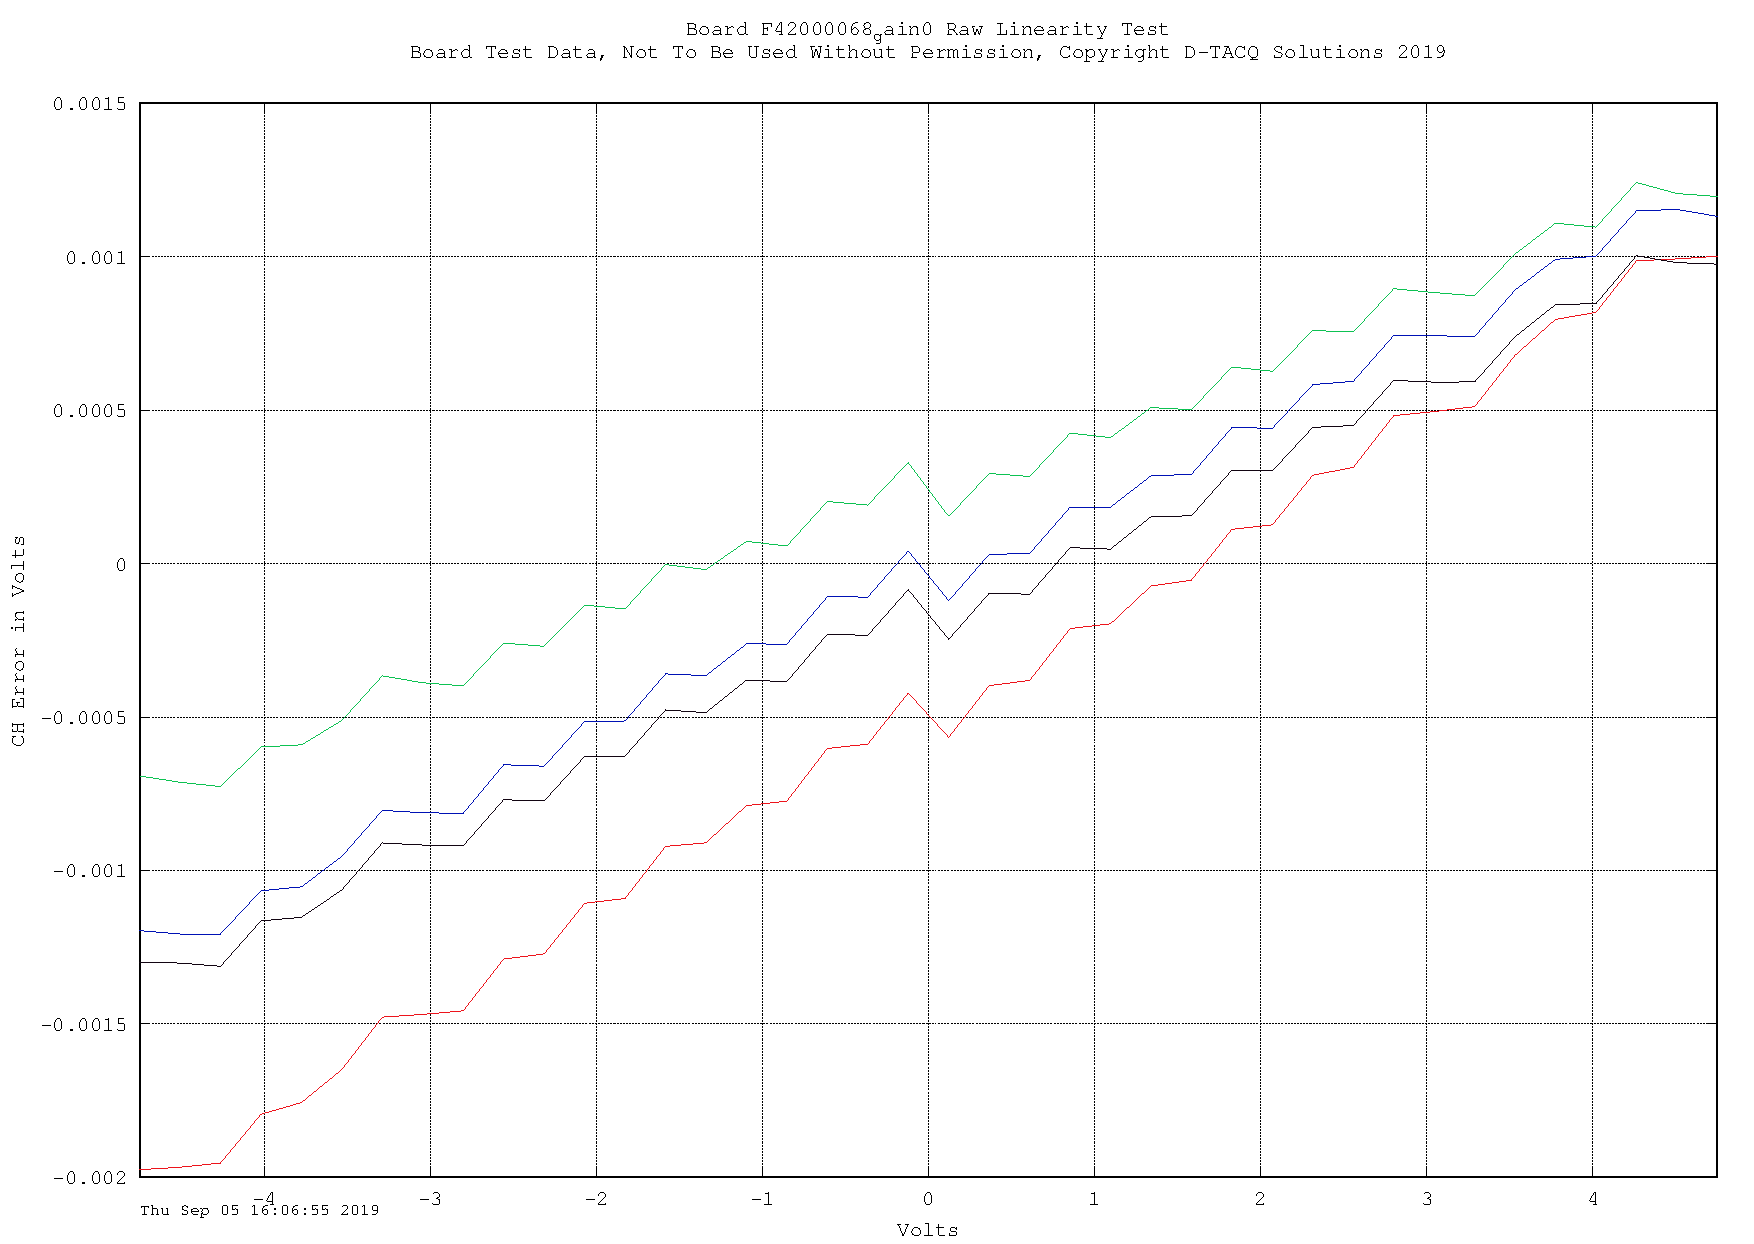
\includegraphics[width=0.9\linewidth]{images/F42000068_gain0_RAW_Linearity_Test}
%		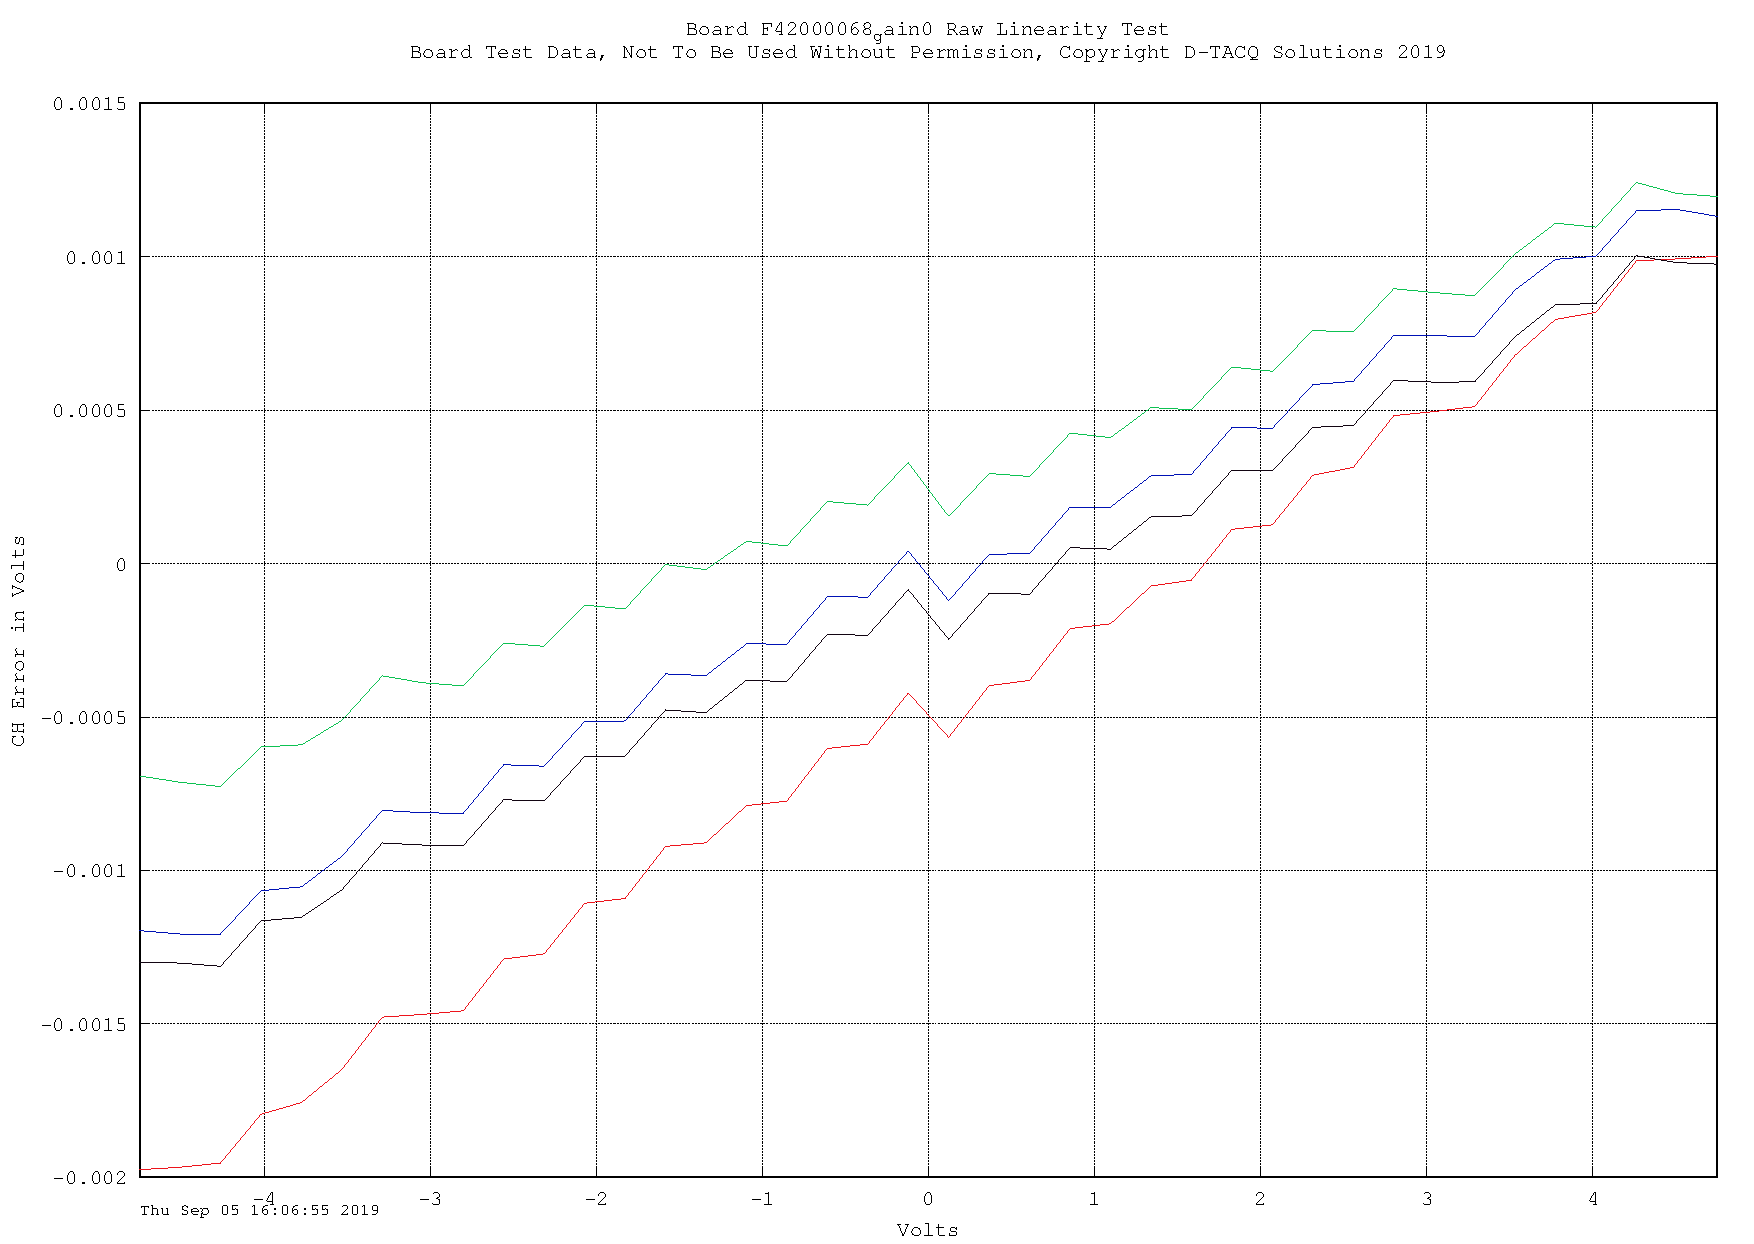
\includegraphics[width=0.9\linewidth, height=50mm]{images/F42000068_gain0_RAW_Linearity_Test} % With height specified
		\caption{Decent Linearity}
		\label{fig:goodlin}
	\end{subfigure}
	\begin{subfigure}{0.5\textwidth}
		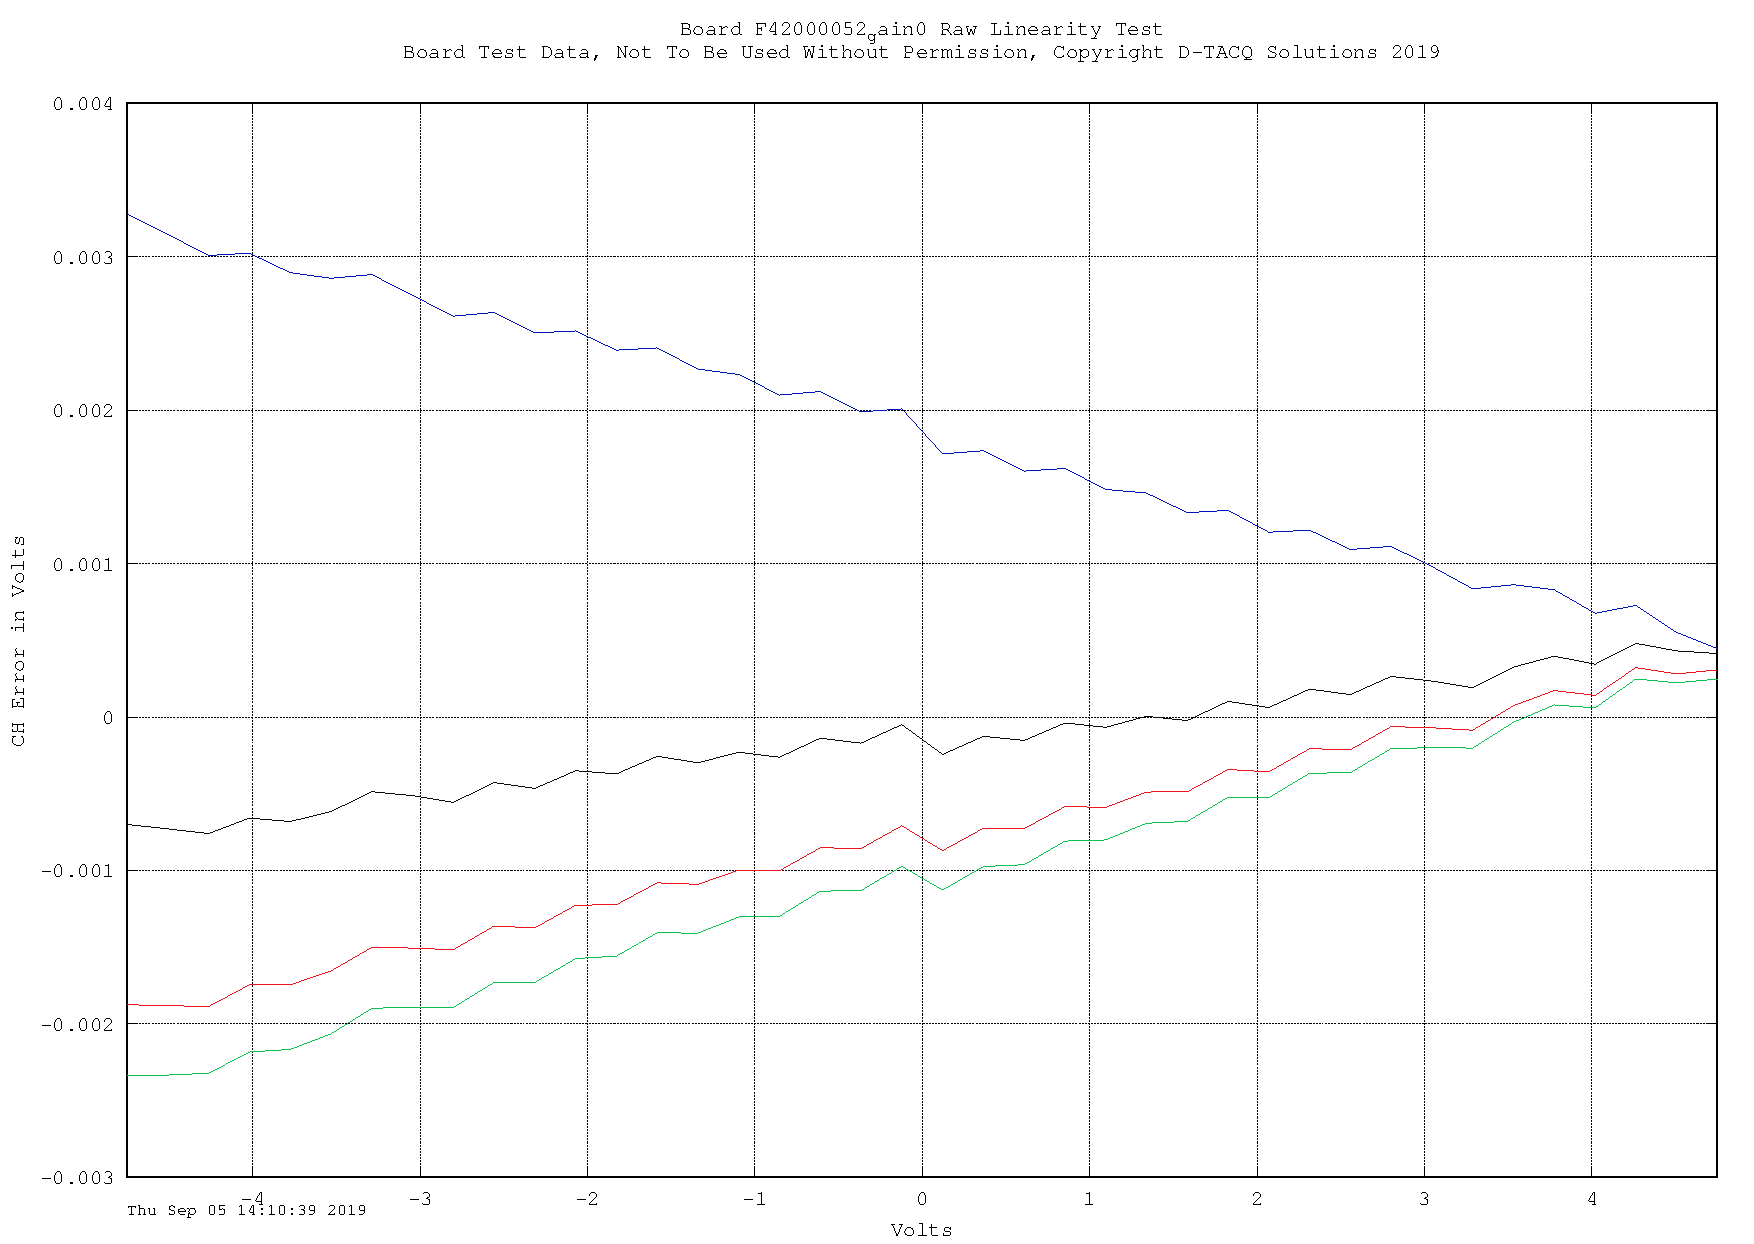
\includegraphics[width=0.9\linewidth]{images/F42000052_gain0_RAW_Linearity_Test}
		\caption{Less Decent Linearity}
		\label{fig:badlin}
	\end{subfigure}
	
	\caption{Linearity Comparison between two AO420 Mezzanines}
	\label{fig:complin}
\end{figure}

Continued lorem ipsum nonsense in order to input a newline to make the next sentence stand out.\\\\
Refer to Figure \ref{fig:goodlin} for an example of somewhat normal DAC linearity on an AO420.
Contrast this with the result in Figure \ref{fig:badlin}.
Here we have two figures side-by-side using the subfigure command. Pretty useful for comparisons.

\section{Section 2}
Let's start this section with another figure.

\begin{figure} [h]
	\centering
	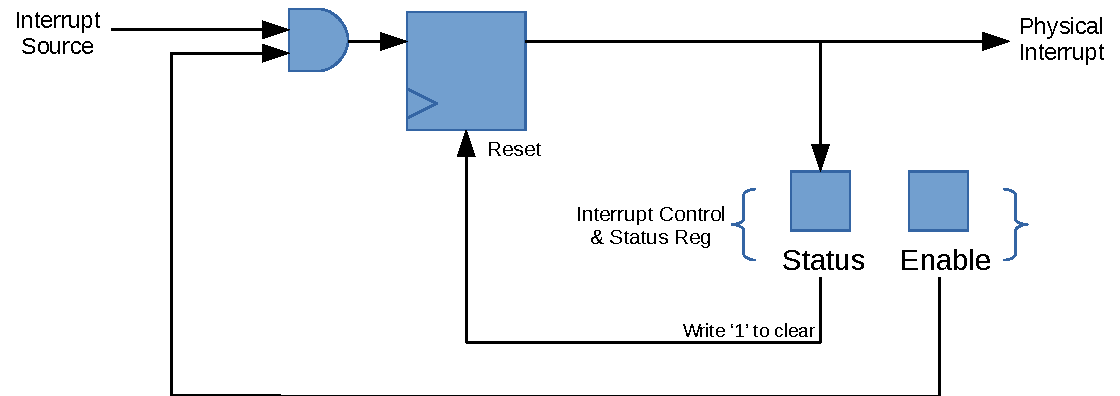
\includegraphics[width=100mm]{images/original_interrupt_style}
	\caption{Simplified logic illustrating the original ACQ400 interrupt style}
	\label{orig_int}
\end{figure}

Here we have an example of a figure all by itself.\\
\lipsum[1]

\section{Section 3}
Let's try a table!

\begin{table}[h]
	\begin{center}
		\begin{tabular}{|c|c|c|c|c|c|}
			
			\hline Frequency (Hz) & Peak Amplitude & Associated DFT Bin & Spectral Loss (dB)\\ 
			\hline 200 & 8 & 200 & 0 \\ 
			\hline 210 & 7.758 & 200 & 0.27 \\ 
			\hline 220 & 6.407 & 200 & 1.93 \\
			\hline 225 & 5.222 & 200 & 3.71 \\
			\hline 230 & 6.269 & 250 & 2.12 \\
			\hline 240 & 7.799 & 250 & 0.22 \\
			\hline 250 & 8 & 250 & 0 \\
			\hline 
		\end{tabular}\\
		\caption{Table of Calculated and Quoted Scallop Losses for Various Windows}
		\label{fig:TableScallop}
	\end{center}
\end{table}


\end{document}
